% Divide and Conquer Part 2 -- Metropolis beamer slides
% Compile: pdflatex divide-and-conquer-2.tex (x2)
\documentclass[10pt,aspectratio=169]{beamer}

\usetheme{metropolis}
\metroset{block=fill, numbering=fraction, progressbar=frametitle}

\usepackage[T1]{fontenc}
\usepackage{amsmath, amssymb}
\usepackage{mathtools}
\usepackage{listings}
\usepackage{booktabs}
\usepackage{tikz}
\usepackage{pgfplots}
\pgfplotsset{compat=1.18}
\usetikzlibrary{arrows.meta, positioning, decorations.pathreplacing, calc, matrix}

% ---- colors -------------------------------------------------------------
\definecolor{mLightBlue}{HTML}{4C72B0}
\definecolor{mGreen}{HTML}{55A868}
\definecolor{mRed}{HTML}{C44E52}
\definecolor{mGray}{HTML}{BFBFBF}
\setbeamercolor{alerted text}{fg=mRed}

% ---- code style ---------------------------------------------------------
\lstdefinestyle{jl}{
  basicstyle=\ttfamily\footnotesize,
  keywordstyle=\color{mRed}\bfseries,
  commentstyle=\color{mGreen}\itshape,
  numberstyle=\tiny\color{mGray},
  showstringspaces=false,
  breaklines=true,
  columns=fullflexible,
  morekeywords={function,for,in,if,else,elseif,end,return,length,while,nothing,push}
}
\lstset{style=jl}

% ---- title --------------------------------------------------------------
\title{Divide and Conquer, Part 2}
\subtitle{Majority Element, Strassen's Algorithm}
\date{}
\author{}

\begin{document}

\maketitle

% =========================================================================
\section{Finding the Majority}

\begin{frame}{The Problem}
  Given $A[1:n]$ whose elements can only be \alert{compared for equality}.

  \bigskip
  \begin{block}{Majority element}
    An element occurring \alert{strictly more than $n/2$ times} in $A$.
  \end{block}

  \bigskip
  \begin{center}
  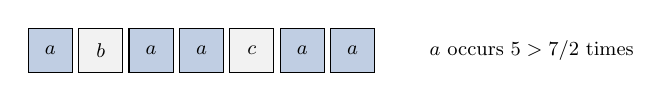
\begin{tikzpicture}[scale=0.8, every node/.style={transform shape}]
    \foreach \v/\fillc [count=\i from 0] in
      {a/mLightBlue!35, b/black!5, a/mLightBlue!35, a/mLightBlue!35,
       c/black!5, a/mLightBlue!35, a/mLightBlue!35} {
      \node[draw, minimum size=7mm, fill=\fillc] at (\i*0.8,0) {\small $\v$};
    }
    \node[right] at (5.9,0) {\small $a$ occurs $5 > 7/2$ times};
  \end{tikzpicture}
  \end{center}

  \bigskip
  \begin{center}
    Naive: count each element against the whole array, giving $O(n^2)$.
  \end{center}
\end{frame}

\begin{frame}{The Key Claim}
  \begin{block}{Claim}
    Let $L, R$ partition $A$. If $A$ has a majority element,
    it is the majority of \alert{$L$ or of $R$} (or both).
  \end{block}

  \bigskip
  \textbf{Proof.} Suppose $z$ is the majority of $A$ but of neither half. Then
  \[
    \text{count}(z, L) + \text{count}(z, R) \le \frac{|L|}{2} + \frac{|R|}{2} = \frac{n}{2},
  \]
  contradicting that $z$ occurs more than $n/2$ times in $A$. $\square$

  \bigskip
  \begin{center}
    So there are only \alert{two candidates} to check.
  \end{center}
\end{frame}

\begin{frame}[fragile]{A Divide-and-Conquer Algorithm}
  Recurse on both halves, then verify each candidate against the full array.

  \begin{lstlisting}
function majority(A)
    n = length(A)
    if n == 0
        return nothing
    elseif n == 1
        return A[1]
    end

    L = A[1:div(n,2)];  R = A[div(n,2)+1:end]
    x = majority(L);    y = majority(R)

    count_x = sum(1 for a in A if a == x)
    count_y = sum(1 for a in A if a == y)

    count_x > n/2 && return x
    count_y > n/2 && return y
    return nothing
end
  \end{lstlisting}
\end{frame}

\begin{frame}{Running Time}
  Two calls of half the size, plus $O(n)$ to count both candidates:

  \begin{alertblock}{}
    \[
      T(n) = 2\,T(n/2) + O(n) \;=\; O(n \log n)
    \]
  \end{alertblock}

  \bigskip
  \begin{center}
    Better than $O(n^2)$. \quad Can we reach $O(n)$?
  \end{center}
\end{frame}

% ---------------------------------------------------------------- improved
\begin{frame}{A Better Idea: Pairing}
  Pair up neighbours. Keep \alert{one copy} of a matching pair, \alert{discard} a mismatched pair.

  \bigskip
  \begin{center}
  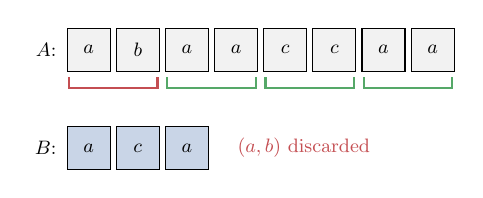
\begin{tikzpicture}[scale=0.78, every node/.style={transform shape}]
    % A
    \node[left] at (-0.4,0.9) {\small $A$:};
    \foreach \v [count=\i from 0] in {a,b,a,a,c,c,a,a} {
      \node[draw, minimum size=7mm, fill=black!5] at (\i*0.8,0.9) {\small $\v$};
    }
    % pair brackets
    \foreach \s in {0,2,4,6} {
      \pgfmathsetmacro{\xa}{\s*0.8-0.32}
      \pgfmathsetmacro{\xb}{\s*0.8+1.12}
      \ifnum\s=0 \def\cc{mRed}\else\def\cc{mGreen}\fi
      \draw[\cc, thick] (\xa,0.45) -- (\xa,0.28) -- (\xb,0.28) -- (\xb,0.45);
    }
    \node[left] at (-0.4,-0.7) {\small $B$:};
    \foreach \v [count=\i from 0] in {a,c,a} {
      \node[draw, minimum size=7mm, fill=mLightBlue!30] at (\i*0.8,-0.7) {\small $\v$};
    }
    \node[right] at (2.3,-0.7) {\small \textcolor{mRed}{$(a,b)$ discarded}};
  \end{tikzpicture}
  \end{center}

  \bigskip
  \begin{center}
    If $m$ is the majority of $A$, then $m$ is the majority of $B$.\\
    \smallskip
    \small The converse fails, so we must verify at the end.
  \end{center}
\end{frame}

\begin{frame}{Why the Majority Survives}
  Let $m$ be the majority of $A$. Among the $n/2$ pairs, let
  \begin{itemize}
    \item $x$ = pairs $(m,m)$, \quad $y$ = pairs with exactly one $m$, \quad $t$ = pairs with no $m$.
  \end{itemize}

  \bigskip
  Then $x + y + t = \dfrac{n}{2}$ and $m$ occurs $2x + y > \dfrac{n}{2}$ times.

  \bigskip
  Subtracting the first from the second:
  \[
    (2x + y) - (x + y + t) > 0 \;\Longrightarrow\; \alert{x > t}.
  \]
\end{frame}

\begin{frame}{Why the Majority Survives}
  In the reduced array $B$:
  \begin{itemize}
    \item each $(m,m)$ pair contributes exactly one $m$ \; $\Rightarrow$ \; $m$ appears $x$ times;
    \item each pair with no $m$ contributes \emph{at most} one element.
  \end{itemize}

  \bigskip
  So $|B| \le x + t$, and since $x > t$,
  \[
    2x > x + t \ge |B|
    \qquad\Longrightarrow\qquad
    x > \frac{|B|}{2}.
  \]

  \bigskip
  \begin{center}
    $m$ is still a majority element of $B$. $\square$
  \end{center}
\end{frame}

\begin{frame}{The Improved Algorithm}
  \begin{enumerate}
    \item If $n$ is odd, test $A[1]$ directly; if it is not the majority, drop it. \hfill $O(n)$
    \bigskip
    \item Pair up neighbours and build $B$ as above. \hfill $O(n)$
    \bigskip
    \item Recurse: $m \leftarrow \texttt{majority}(B)$, where $|B| \le n/2$.
    \bigskip
    \item Verify $m$ against the \alert{original} $A$. \hfill $O(n)$
  \end{enumerate}

  \bigskip
  \begin{alertblock}{}
    \[
      T(n) = T(n/2) + O(n) \;=\; O(n)
    \]
  \end{alertblock}
\end{frame}

\begin{frame}[fragile]{Implementation}
  \begin{lstlisting}
function majority_fast(A)
    n = length(A)
    n == 0 && return nothing
    n == 1 && return A[1]

    C = A                        # handle odd length
    if n % 2 == 1
        count = sum(1 for a in A if a == A[1])
        count > n/2 && return A[1]
        C = @view A[2:end]
    end

    B = Vector{eltype(A)}()      # reduced array
    for i in 1:2:length(C)
        C[i] == C[i+1] && push!(B, C[i])
    end

    x = majority_fast(B)         # recurse, then verify
    if x !== nothing && sum(1 for a in A if a == x) > n/2
        return x
    end
    return nothing
end
  \end{lstlisting}
\end{frame}

% =========================================================================
\section{Strassen's Algorithm}

\begin{frame}{Matrix Multiplication}
  For $n \times n$ matrices $X$ and $Y$, the product $Z = XY$ has
  \[
    Z_{ij} = \sum_{k=1}^{n} X_{ik} Y_{kj}.
  \]

  \bigskip
  \begin{center}
  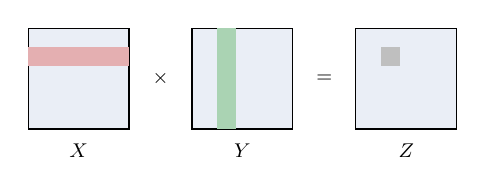
\begin{tikzpicture}[scale=0.8, every node/.style={transform shape}]
    \draw[fill=mLightBlue!12] (0,0) rectangle (1.6,1.6);
    \fill[mRed!45] (0,1.0) rectangle (1.6,1.3);
    \node at (0.8,-0.35) {\small $X$};
    \node at (2.1,0.8) {\small $\times$};
    \draw[fill=mLightBlue!12] (2.6,0) rectangle (4.2,1.6);
    \fill[mGreen!50] (3.0,0) rectangle (3.3,1.6);
    \node at (3.4,-0.35) {\small $Y$};
    \node at (4.7,0.8) {\small $=$};
    \draw[fill=mLightBlue!12] (5.2,0) rectangle (6.8,1.6);
    \fill[mGray] (5.6,1.0) rectangle (5.9,1.3);
    \node at (6.0,-0.35) {\small $Z$};
  \end{tikzpicture}
  \end{center}

  \bigskip
  \begin{center}
    $n^2$ entries $\times$ $O(n)$ each $= O(n^3)$ for the naive method.
  \end{center}
\end{frame}

\begin{frame}{Block Multiplication}
  Matrix multiplication works \alert{blockwise} (assume $n$ is a power of 2):
  \[
    \begin{bmatrix} A & B \\ C & D \end{bmatrix}
    \cdot
    \begin{bmatrix} E & F \\ G & H \end{bmatrix}
    =
    \begin{bmatrix} AE + BG & AF + BH \\ CE + DG & CF + DH \end{bmatrix}
  \]

  \bigskip
  That is \alert{8} multiplications of $(n/2) \times (n/2)$ blocks, plus $O(n^2)$ of additions:
  \[
    T(n) = 8\,T(n/2) + O(n^2)
    \;\overset{\text{Master}}{=}\; O(n^3).
  \]

  \bigskip
  \begin{center}
    No better than the naive algorithm.
  \end{center}
\end{frame}

\begin{frame}{Exercise}
  Verify block multiplication on this example, using blocks of size 2.

  \bigskip
  \[
    \begin{bmatrix}
      1 & 2 & 3 & 2\\
      5 & 2 & 1 & 0 \\
      1 & 1 & 1 & 0 \\
      2 & 3 & 5 & 7
    \end{bmatrix}
    \cdot
    \begin{bmatrix}
      1 & 0 & 0 & 1\\
      1 & 1 & 2 & 1 \\
      1 & 2 & 3 & 4 \\
      5 & 6 & 7 & 8
    \end{bmatrix}
    = \; \ldots
  \]
\end{frame}

\begin{frame}{Solution}
  With $A = \begin{bsmallmatrix}1&2\\5&2\end{bsmallmatrix}$,
  $B = \begin{bsmallmatrix}3&2\\1&0\end{bsmallmatrix}$,
  $E = \begin{bsmallmatrix}1&0\\1&1\end{bsmallmatrix}$,
  $G = \begin{bsmallmatrix}1&2\\5&6\end{bsmallmatrix}$:
  \[
    AE + BG
    = \begin{bmatrix}3&2\\7&2\end{bmatrix}
    + \begin{bmatrix}13&18\\1&2\end{bmatrix}
    = \begin{bmatrix}16&20\\8&4\end{bmatrix}.
  \]

  \bigskip
  Multiplying the full $4 \times 4$ matrices directly gives the same top-left block:
  \[
    \begin{bmatrix}
      16 & 20 & \cdot & \cdot \\
       8 &  4 & \cdot & \cdot \\
     \cdot & \cdot & \cdot & \cdot \\
     \cdot & \cdot & \cdot & \cdot
    \end{bmatrix}
  \]

  \begin{center}
    \small The other three blocks check out the same way.
  \end{center}
\end{frame}

\begin{frame}{Strassen's Trick}
  Seven products instead of eight:

  \bigskip
  \begin{center}
  \begin{minipage}{0.42\textwidth}
    \begin{itemize}
      \item $P_1 = A(F-H)$
      \item $P_2 = (A+B)H$
      \item $P_3 = (C+D)E$
      \item $P_4 = D(G-E)$
    \end{itemize}
  \end{minipage}\hfill
  \begin{minipage}{0.5\textwidth}
    \begin{itemize}
      \item $P_5 = (A+D)(E+H)$
      \item $P_6 = (B-D)(G+H)$
      \item $P_7 = (A-C)(E+F)$
    \end{itemize}
  \end{minipage}
  \end{center}

  \bigskip
  Each sum or difference costs $O(n^2)$, so each $P_i$ costs $T(n/2) + O(n^2)$.
\end{frame}

\begin{frame}{Reassembling the Product}
  \[
    \begin{bmatrix} AE + BG & AF + BH \\ CE + DG & CF + DH \end{bmatrix}
  \]

  \bigskip
  \begin{itemize}
    \item $AE + BG = P_5 + P_4 - P_2 + P_6$
    \item $AF + BH = P_1 + P_2$
    \item $CE + DG = P_3 + P_4$
    \item $CF + DH = P_1 + P_5 - P_3 - P_7$
  \end{itemize}

  \bigskip
  \begin{alertblock}{}
    \[
      T(n) = 7\,T(n/2) + O(n^2)
      \;=\; O(n^{\log_2 7}) \approx O(n^{2.81})
    \]
  \end{alertblock}
\end{frame}

\begin{frame}{$8$ versus $7$}
  \begin{center}
  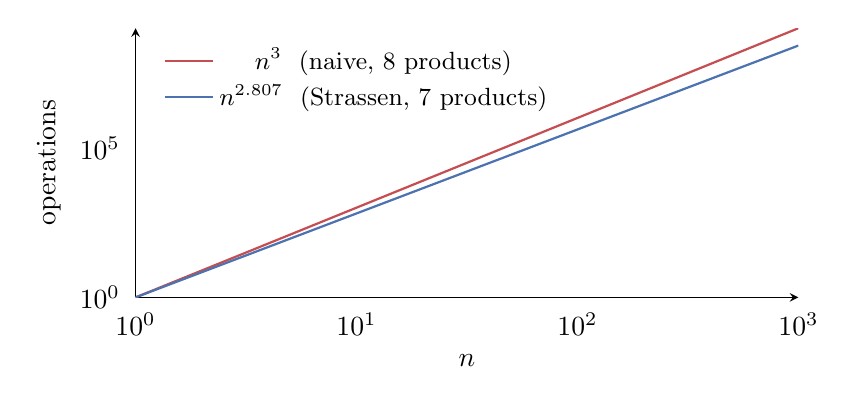
\begin{tikzpicture}
    \begin{axis}[
      width=10cm, height=5cm,
      domain=1:1000, samples=100,
      axis lines=left, tick style={draw=none},
      xlabel={$n$}, ylabel={operations},
      ymode=log, xmode=log,
      legend pos=north west,
      legend style={draw=none, fill=none, font=\small},
    ]
      \addplot[thick, mRed] {x^3};
      \addlegendentry{$n^3$ \ (naive, 8 products)}
      \addplot[thick, mLightBlue] {x^2.807};
      \addlegendentry{$n^{2.807}$ \ (Strassen, 7 products)}
    \end{axis}
  \end{tikzpicture}
  \end{center}

  \begin{center}
    \small One fewer multiplication per level, compounded over $\log_2 n$ levels.
  \end{center}
\end{frame}

\begin{frame}[fragile]{Implementation}
  \begin{lstlisting}
function strassen(A::AbstractMatrix, B::AbstractMatrix)
    n = size(A, 1)
    n <= 32 && return A * B          # base case

    mid = n div 2
    A11, A12 = @view(A[1:mid, 1:mid]),     @view(A[1:mid, mid+1:end])
    A21, A22 = @view(A[mid+1:end, 1:mid]), @view(A[mid+1:end, mid+1:end])
    B11, B12 = @view(B[1:mid, 1:mid]),     @view(B[1:mid, mid+1:end])
    B21, B22 = @view(B[mid+1:end, 1:mid]), @view(B[mid+1:end, mid+1:end])

    P1 = strassen(A11, B12 - B22);   P2 = strassen(A11 + A12, B22)
    P3 = strassen(A21 + A22, B11);   P4 = strassen(A22, B21 - B11)
    P5 = strassen(A11 + A22, B11 + B22)
    P6 = strassen(A12 - A22, B21 + B22)
    P7 = strassen(A11 - A21, B11 + B12)

    C = Matrix{eltype(A)}(undef, n, n)
    C[1:mid, 1:mid]         .= P5 + P4 - P2 + P6
    C[1:mid, mid+1:end]     .= P1 + P2
    C[mid+1:end, 1:mid]     .= P3 + P4
    C[mid+1:end, mid+1:end] .= P1 + P5 - P3 - P7
    return C
end
  \end{lstlisting}
\end{frame}

\begin{frame}{In Practice}
  \begin{itemize}
    \item Large constant factors and numerical instability.
    \item Better algorithms exist for sparse matrices.
    \item Real implementations switch to the naive method below a threshold.
  \end{itemize}

  \bigskip
  \begin{center}
    Still a beautiful example of what divide-and-conquer buys you.
  \end{center}

  \bigskip
  \begin{center}
    \small Fast matrix multiplication is still active research,\\
    the current best is $O(n^{2.3728596})$ (as of 2024).
  \end{center}
\end{frame}

% =========================================================================
\begin{frame}[standout]
  Questions?
\end{frame}

\end{document}
